% This template was initially provided by Dulip Withanage.
% Modifications for the database systems research group
% were made by Conny Junghans,  Jannik Strötgen and Michael Gertz

\documentclass[
     12pt,         % font size
     a4paper,      % paper format
     BCOR=10mm,     % binding correction
     DIV=14,        % stripe size for margin calculation
     liststotoc,   % table listing in toc
     bibtotoc,     % bibliography in toc
%     idxtotoc,     % index in toc
     parskip=half,       % paragraph skip instead of paragraph indent
     openright
     ]{scrreprt}

%%%%%%%%%%%%%%%%%%%%%%%%%%%%%%%%%%%%%%%%%%%%%%%%%%%%%%%%%%%%

% PACKAGES:

% Input and font encoding
\usepackage{lmodern}
\usepackage[utf8]{inputenc}
\usepackage[T1]{fontenc}
% Index-generation
\usepackage{makeidx}
% Einbinden von URLs:
\usepackage{url}
% Special \LaTex symbols (e.g. \BibTeX):
%\usepackage{doc}
% Include Graphic-files:
\usepackage{graphicx}
% Include doc++ generated tex-files:
%\usepackage{docxx}
% Include PDF links
%\usepackage[pdftex, bookmarks=true]{hyperref}

% Fuer anderthalbzeiligen Textsatz
\usepackage{setspace}

% for subfigures (i.e. multiple images side-by-side)
\usepackage{subcaption}

\usepackage{amsmath} %for stuff over arrows
\newcommand{\Mod}[1]{\ \mathrm{mod}\ #1} %new command for mod's without the leading spaces

\usepackage{amsthm}
\theoremstyle{remark}
\newtheorem*{remark}{Remark}

%I switched to BibLatex
\usepackage[backend=biber]{biblatex}
\addbibresource{references.bib}

% hyperrefs in the documents
\usepackage[bookmarks=true,colorlinks,pdfpagelabels,pdfstartview = FitH,bookmarksopen = true,bookmarksnumbered = true,linkcolor = black,plainpages = false,hypertexnames = false,citecolor = black,urlcolor=black]{hyperref}
%\usepackage{hyperref}

%%%%%%%%%%%%%%%%%%%%%%%%%%%%%%%%%%%%%%%%%%%%%%%%%%%%%%%%%%%%

% OTHER SETTINGS:

% Pagestyle:
\pagestyle{headings}

%caption spacing
\setlength{\abovecaptionskip}{3pt}


\begin{document}

% TITLE:
\pagenumbering{roman}
\begin{titlepage}


\vspace*{1cm}
\begin{center}
\vspace*{3cm}
\textbf{
\Large Heidelberg University\\
\smallskip
\Large Faculty of Mathematics and Computer Science\\
\smallskip
\Large Interdisciplinary Center for Scientific Computing\\
\smallskip
\Large Scientific Software Center\\
\smallskip
}

\vspace{3cm}

\textbf{\large Bachelor Thesis}

\vspace{0.5\baselineskip}
{\huge
\textbf{Viability Evaluation of Homomorphic Encryption in Machine Learning}
}
\end{center}

\vfill

{\large
\begin{tabular}[l]{ll}
Name: & Julian Partanen\\
Matriculation Number: & 4204806\\
Supervisor: & Dr. Dominic Kempf\\
Submission Date: & December 02, 2025
\end{tabular}
}

\end{titlepage}

% Add a brief summary of your topic and contributions (Zusammenfassung) in German *and* in English:
% This file contains an abstract of your thesis, with approximaltely 300-500 words

\chapter*{Abstract}
The abstract has to be given in German \textbf{and} English. It should
be between half a page and one page in length. It should cover in a
readable and comprehensive style the context of the thesis, the
problem setting, the objectives, and the methods developed in this
thesis as well as key insights and results.


% This file contains the German version of your abstract, with about 300-500 words

Die Zusammenfassung muss auf Deutsch \textbf{und} auf Englisch geschrieben
werden. Die Zusammenfassung sollte zwischen einer halben und einer
ganzen Seite lang sein. Sie soll den Kontext der Arbeit, die
Problemstellung, die Zielsetzung und die entwickelten Methods sowie
Erkenntnisse bzw.~Ergebnisse übersichtlich und verständlich
beschreiben.


% MAIN PART:
% Table of contents (Inhaltsverzeichnis)
\tableofcontents
\cleardoublepage
\pagenumbering{arabic}

%%%%%%%%%%%%%%%%%%%%%%%%%%%%%%%%%%%%%%%%%%%%%%%%%%%%%%%%%%%%%%%
% Here, the actual content of your thesis begins
% You can either put all the text here or use individual files to store the chapters of your thesis.
% Below are templates for both alternatives.

\chapter{Introduction}\label{intro}

introduction stuff

\section{Motivation}

I'm motivated!

\section{Goals}

Challenges and goals

\section{Structure}

bla

\chapter{Background}

The topic of this thesis falls into an overlap between the fields of cryptography and machine learning, and as such we will first introduce some concepts from both fields in this chapter. We will not assume anything more than surface-level knowledge in any of the two fields from the reader.

\section{Cryptography Concepts and FHE}

\subsection{Basic Notation and Phrases}

Throughout this work we will use some of the following notations and phrases that are also commonly encountered in other cryptography-related works. We will introduce these concepts informally aiming for a basic understanding of them while linking to formal definitions.

First we need to introduce the concept of randomness in the context of computational theory. For this we will use the definitions of Anjeev Arora's and Boaz Barak's "Computational Complexity: A Modern Approach" \cite{arora_computational_2009}. Many algorithms in Cryptography rely inherently on randomness and thus cannot be modeled by a standard deterministic Turing Machine (TM) with polynomial programs. Instead we need to model their computation using the Probabilistic Turing Machine (PTM) which is an extension of the TM. In contrast to the TM which only has one transition function $\delta$, the PTM has two transition functions $\delta_0$ and $\delta_1$ and chooses at each step at random which one to apply, with probability half to apply $\delta_0$ and half to apply $\delta_1$.

Similarly how $\mathbf{P}$ is the class of decision problems that are solvable in polynomial time by a TM, $\mathbf{BPP}$ is the class of decision problems that are solvable in polynomial time by a PTM. Note that since the TM is a special case of the PTM (the one where $\delta_0 = \delta_1$), and since it is possible to simulate all branches of a PTM with a TM in time $2^{poly(n)}$ it holds that $\mathbf{P} \subseteq \mathbf{BPP} \subseteq \mathbf{EXP}$ (see chapter 7.1 in \cite{arora_computational_2009}).

An alternative definition of a PTM would be to add a second tape to a TM which includes bits that are results of fair coin tosses, i.e. each symbol on the second tape is chosen mutually independent and uniformly at random from the set $\{ 0, 1 \}$, and then the tape is fed to a TM in addition to the regular input tape. From this viewpoint comes a phrasing of referring to the randomness in cryptographic algorithms like encrypt or key generation functions as 'coins'. These independent random coin-flips can be viewed as an implicit input to any such algorithm, and are in practice most commonly obtained by pseudo-random number generators.

Furthermore, as introduced in the lecture notes of Mihir Bellare and Phillip Rogaway \cite{bellare_introduction_2005} in chapter 1.3, we will use the following notation to mean that $i$ is a value chosen uniformly at random from the set $\mathcal{S}$: $i \xleftarrow{\$} \mathcal{S}$. This notation can also be used for algorithms, e.g. $i \xleftarrow{\$} \text{Encrypt}$ which can be viewed as $i$ being a random value from the image of 'Encrypt', or a random result of all possible branches of the PTM-equivalent of the 'Encrypt' algorithm chosen uniformly at random. The \$ denotes the random coins used as input. Note that some literature may also use $R$ instead of \$.

\section{Machine Learning Concepts and Model Types}

\chapter{Method}

In this chapter we will describe the experiment setup used to measure various trade-offs of homomorphic encryption in different machine learning scenarios. We will describe the technologies and general methodology as well as all the different datasets and model architectures used.

\section{Technological Overview}

The source code of all experiments described in this thesis is open-source and available on GitHub \cite{partanen_julianfpfhe-experiments_2025}. The repository includes a README file with some basic instructions in how to run the experiments. This means that the reader may generate every data point or graph in this thesis themselves. The absolute numbers will differ because of hardware and software environment differences, but the relative numbers as well as general findings should thus be reproducible by anyone .

The experiments were implemented in Python, the de facto standard language in the field of machine learning. We have added astral's \emph{uv} \cite{astral_uv_nodate} as a project and dependency management tool to make running the script with all necessary dependencies easier and to pinpoint all dependencies to a specific version to increase reproducibility.

We defined a common interface for all experiments as well as datasets to ease their implementation, reduce code duplication, and to ensure to only change desired attributes between different experiments to increase comparability.

For generating result data we used Python's statistics and csv modules as well as \emph{matplotlib} \cite{noauthor_matplotlib_nodate} to generate all graphics. The graph generation runs independently from the experiment execution which allows redrawing graphs of existing experiment results to for example change the styling of graphs after the fact.

The python package also uses \emph{click} \cite{pallets_welcome_nodate} to add an easy-to-use CLI to be able to adjust parameters like execution repetitions, which experiment-dataset combinations should be executed, or which graphs should be generated.

\section{Datasets}

We used a variation of datasets across different classification problems commonly solved with a machine learning approach. Some of these datasets are synthetic for maximum control over their characteristics to specifically measure a models behavior under certain conditions, while others are real-world datasets that we used to measure how well the models perform solving a variety of real-world problems, mimicking a production deployment of a homomorphic machine learning setup as much as possible.

All datasets use single-precision floating point numbers to store feature vectors to make them compatible with all concrete-ml models since some of these models don't support double-precision for their training data. We made this choice to increase comparability both between FHE and non-FHE executions as well as across different model architectures and since the accuracy trade-off should be almost non-existing.

\subsection{XOR problem}

We handcrafted this tiny dataset for code testing with faster iterations as well as quick experiment runs, however it proofed to also be a good metric for how a model handles non-linearity in a dataset, and if a model is able to fit to problem with a very small training set.

\begin{figure}[h]
    \begin{center}
        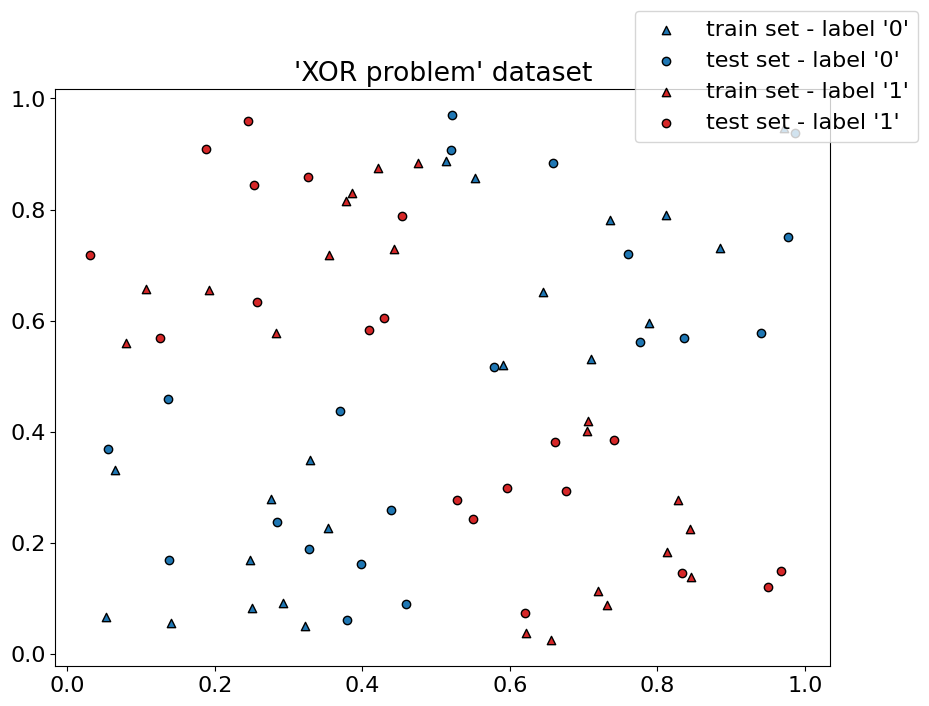
\includegraphics[width=0.65\textwidth]{figures/'XOR problem' dataset.png}
    \end{center}
    \caption{A plot of the feature space of the 'XOR problem' dataset, including both train and test sets}
    \label{fig:xor_problem_plot}
\end{figure}

The dataset's feature vectors are 2-dimensional. The label is 1 if and only if one of the features is closer to 0.75 than to 0.25 while the other is closer to 0.25 than to 0.75. Conversely if both features are approximately the same then the label is 0.

As the name suggests this mimics the boolean XOR operator, with some differences: The inputs are 0.25 and 0.75 instead of 0 and 1 to keep them between 0 and 1 even with noise applied. Since some models require more than just 4 samples we also repeated each of them 10 times for both the training and test set resulting in a total of 40 samples each. To make these repeated samples unique and to add meaningful differences between the training and test set we added some noise to all samples in the form of a random number drawn from an unique distribution between $\pm 0.24$.

The result can be seen in \ref{fig:xor_problem_plot}: A feature space with 4 feature clusters, arranged in a way that makes it impossible for a linear model to separate with an accuracy higher than 75\%. This makes this dataset great in ensuring that more complex non-linear model actually come with an accuracy improvement.

\subsection{Synthetic}

This dataset is a generated at random using scikit-learn's \emph{make\_classification} function. It includes 250 samples, of which 150 are used for training, and 100 for testing. Both classes have only one cluster, making it linearly separable and thus even very simple models should have no problem achieving high accuracy scores on this dataset.

\begin{figure}[h]
    \centering
    \begin{subfigure}[t]{0.32\textwidth}
        \centering
        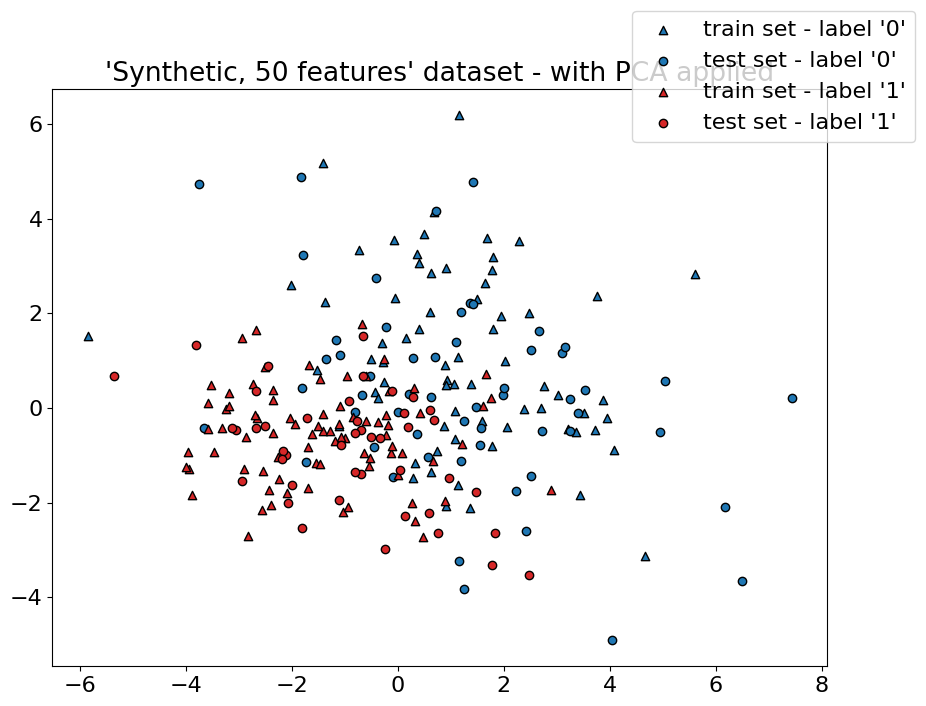
\includegraphics[width=0.95\textwidth]{figures/'Synthetic, 50 features' dataset - with PCA applied.png}
        \caption{50-dim}
    \end{subfigure}
    \begin{subfigure}[t]{0.32\textwidth}
        \centering
        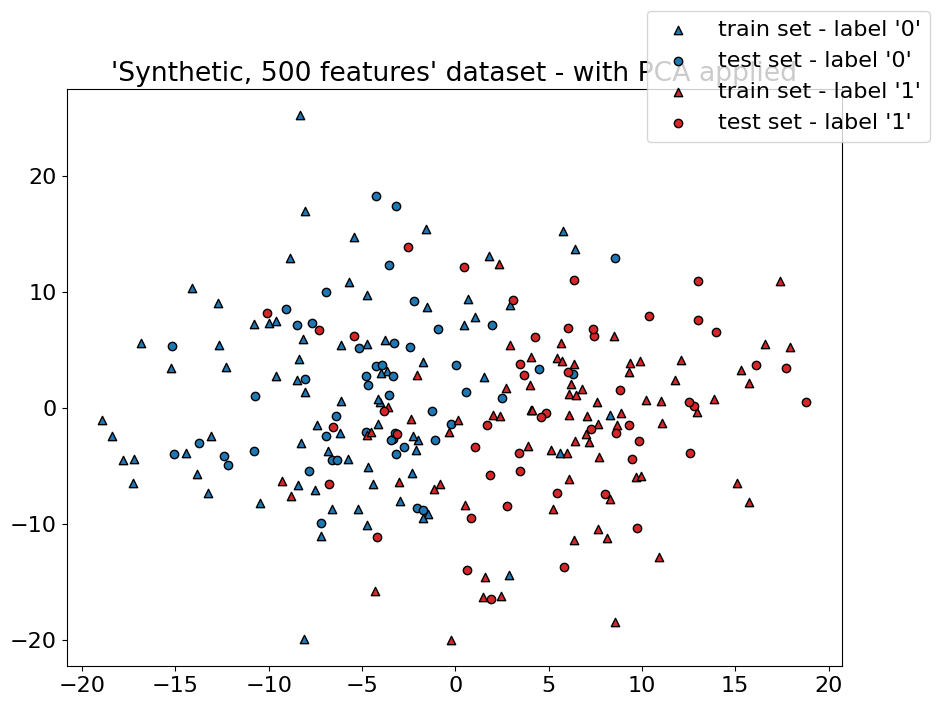
\includegraphics[width=0.95\textwidth]{figures/'Synthetic, 500 features' dataset - with PCA applied.png}
        \caption{500-dim}
    \end{subfigure}
    \begin{subfigure}[t]{0.32\textwidth}
        \centering
        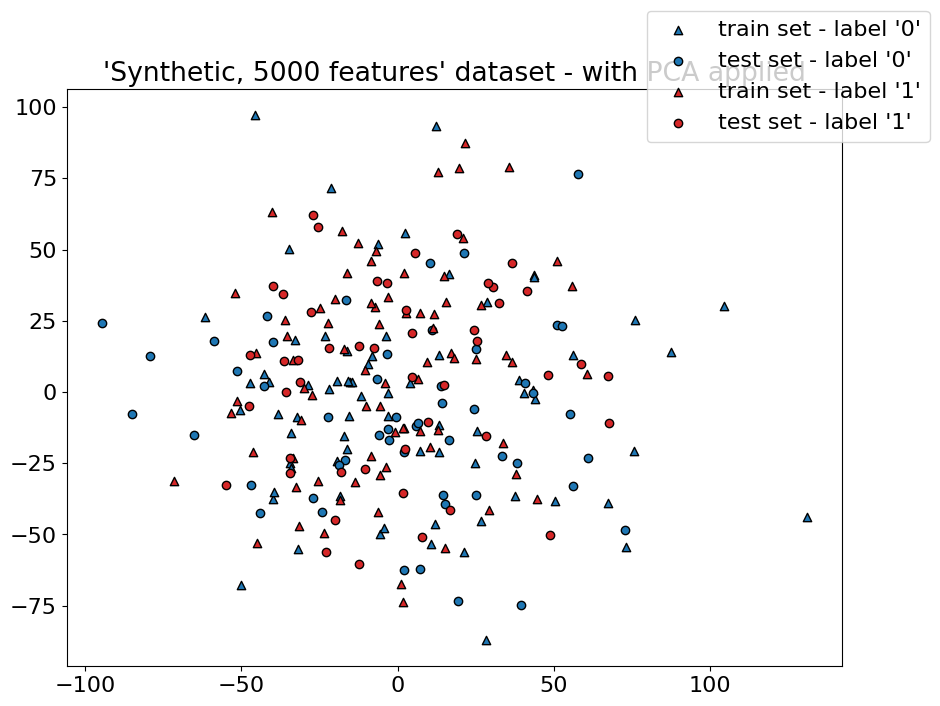
\includegraphics[width=0.95\textwidth]{figures/'Synthetic, 5000 features' dataset - with PCA applied.png}
        \caption{5000-dim}
    \end{subfigure}
    \caption{Plots showing the feature space of three of our seven variations of the 'Synthetic' dataset, PCA-reduced.}
    \label{fig:synthetic_plot}
\end{figure}

The amount of features in this dataset is variable which allows us to specifically isolate the impact of feature size on model runtime and performance. We start with 50-dimensional features, and gradually increase the dimensionality up to 5000, resulting in a total of 7 different variations of this dataset. For each variation, only 10\% of the features are actually informative of the sample's label, while the other 90\% are just generated at random independently from the true labels. This mainly tests a models resistance to overfitting.

The result can be seen in \ref{fig:synthetic_plot}. Please note that in contrast to the 2-dimensional 'XOR problem' dataset we had to map these high dimensional features to 2 dimensions in order to plot them. For this we used scikit-learn's principal component analysis (PCA) implementation. Please note that by doing this, the visual representation of the dataset isn't accurate, for example in the plots it doesn't appear to be separable even though in reality it is. The high amount of uninformative dimensions contributes to this effect.

\subsection{SMS Spam}

This is our first real-world dataset and we will use it to represent the use-case of document classification during our experiments. The SMS Spam dataset was developed by Tiago A. Almeida, José María Gómez and Akebo Yamakami \cite{almeida_contributions_2011} and consists of text messages that are labeled as either ham (label '0') or spam (label '1').

\begin{figure}[h]
    \centering
    \begin{subfigure}[t]{0.32\textwidth}
        \centering
        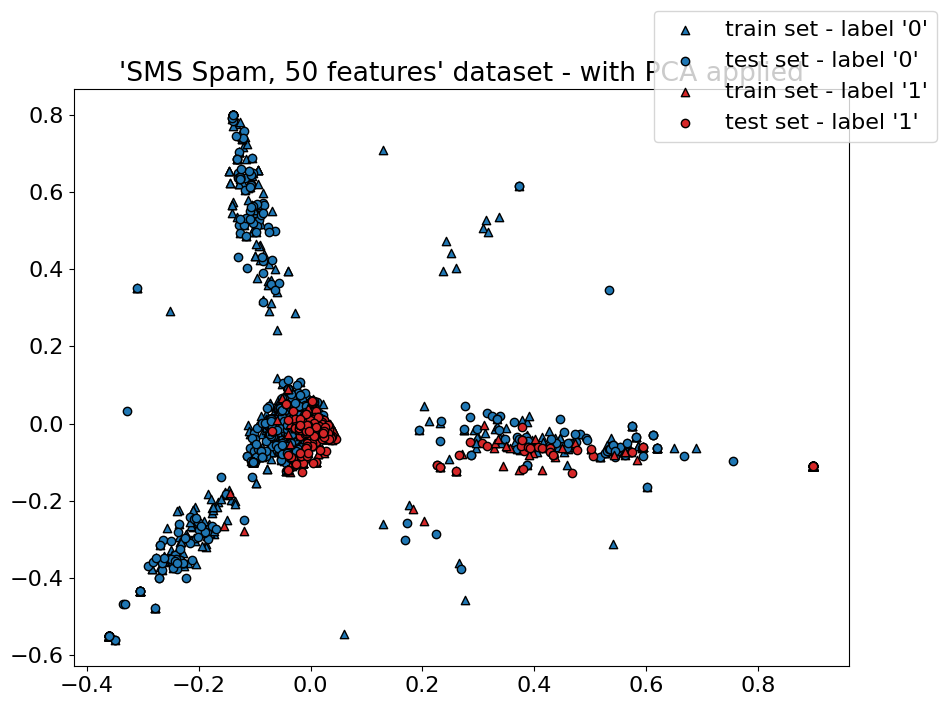
\includegraphics[width=0.95\textwidth]{figures/'SMS Spam, 50 features' dataset - with PCA applied.png}
        \caption{50-dim}
    \end{subfigure}
    \begin{subfigure}[t]{0.32\textwidth}
        \centering
        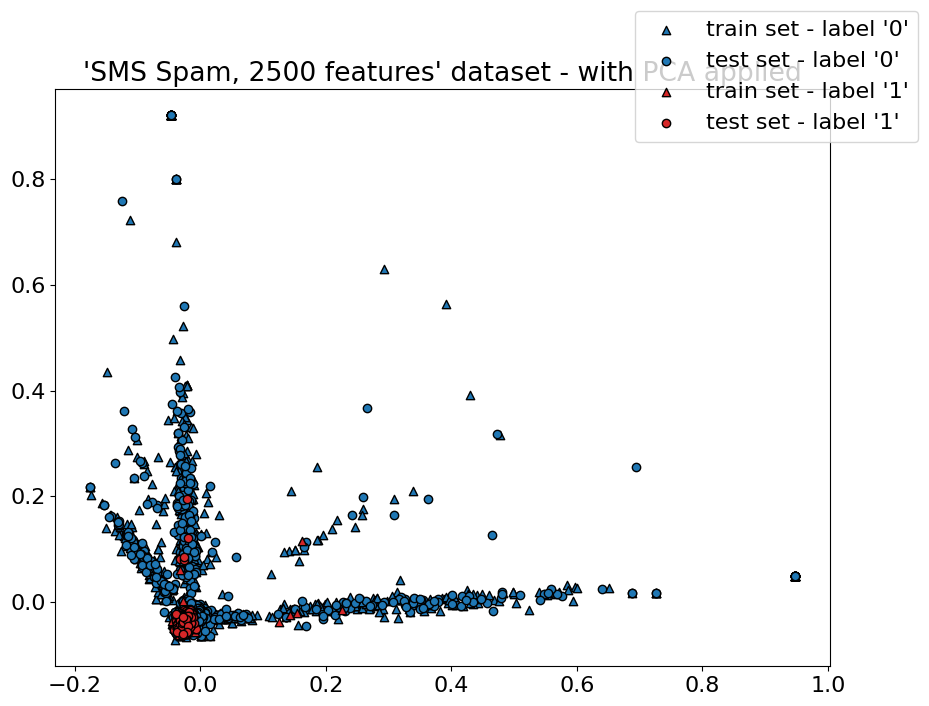
\includegraphics[width=0.95\textwidth]{figures/'SMS Spam, 2500 features' dataset - with PCA applied.png}
        \caption{2500-dim}
    \end{subfigure}
    \begin{subfigure}[t]{0.32\textwidth}
        \centering
        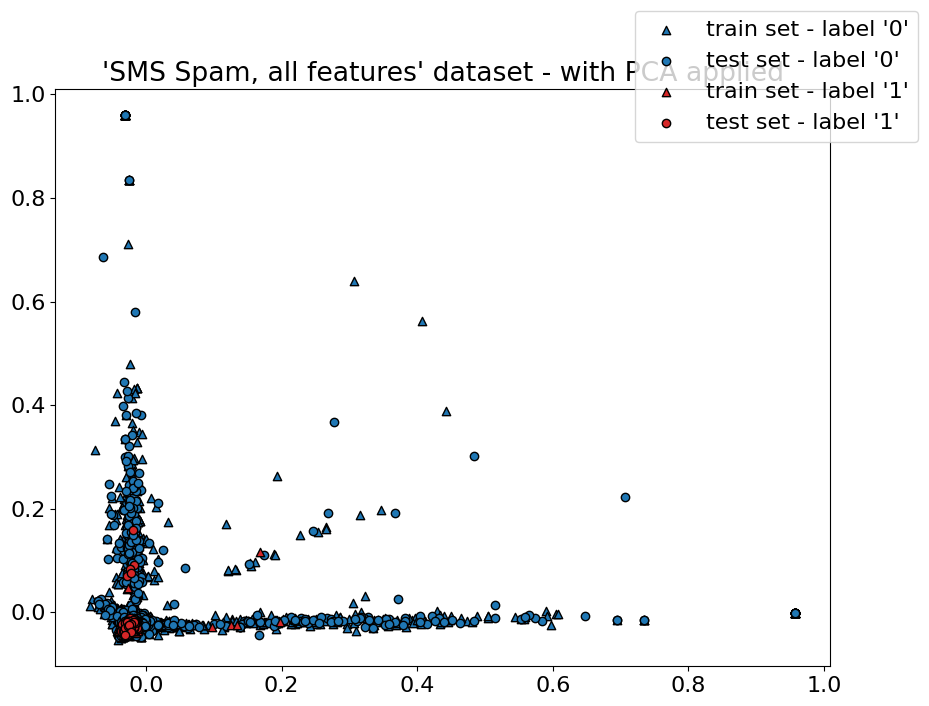
\includegraphics[width=0.95\textwidth]{figures/'SMS Spam, all features' dataset - with PCA applied.png}
        \caption{All features}
    \end{subfigure}
    \caption{Plots showing the feature space of three of our eight variations of the 'SMS Spam' dataset, PCA-reduced.}
    \label{fig:sms_spam_plot}
\end{figure}

To extract feature vectors from the documents we use scikit-learn's TF-IDF Vectorizer while filtering English stop words. Similarly to the 'Synthetic' dataset we also have different variations of this dataset with different feature dimensions ranging from 50 to 5000, as well as one variation which includes all 8444 features. Limiting the amount of features was achieved by ordering the features by term frequency across the corpus and only considering the top x.

Like with the 'Synthetic' dataset we also performed a 60/40 train/test set split which resulted in a dataset size of 3344 and 2230 samples for the training and testing sets respectively.

The result can be seen in \ref{fig:sms_spam_plot}. The same limitation regarding PCA as mentioned for the 'Synthetic' dataset applies here as well.

\include{results}
\chapter{Conclusion and Outlook}
\label{chap:concl}

mooore time

%%%%%%%%%%%%%%%%%%%%%%%%%%%%%%%%%%%%%%%%%%%%%%%%%%%%%%%%%%%%

% List of figures (Abbildungsverzeichnis):
\listoffigures

% List of tables (Tabellenverzeichnis):
%\listoftables

% References (Literaturverzeichnis):
% a) Style (with abbreviations: use alpha):
% see
% https://de.wikibooks.org/wiki/LaTeX-W%C3%B6rterbuch:_bibliographystyle
% for the different formats and styles

%\bibliographystyle{plainnat}
% b) The File:
%\bibliography{references}

%I switched to BibLatex
\printbibliography

\end{document}
